\documentclass[english]{article}

\usepackage{graphicx}
\usepackage{grffile}
\usepackage{babel,blindtext}
\usepackage{parskip}
\textwidth = 426pt
\oddsidemargin = 17pt


\title{Cos301 : Software Requirements Specification\\
	for the ...... System\\
	}
\date{\today}
\graphicspath{{Pictures/}}

\begin{document}
	\maketitle
	\begin{figure}[!t]
		
\includegraphics{up_logo.png}
	\end{figure}
	\begin{minipage}{0.4\textwidth}
		\begin{flushleft} \large
			\textbf{NAMES:}\\[0.4cm]
			Mufamadi {Khodani}
			Mathe {Musa}
		\end{flushleft}
	\end{minipage}
	\begin{minipage}{0.4\textwidth}
		\begin{flushright} \large
			\textbf{STUDENT NUMBER:} \\[0.4cm]
			u14197520
			u15048030
		\end{flushright}
	\end{minipage}


	
	\pagenumbering{gobble}
	\newpage

	\tableofcontents
	\newpage

	\pagenumbering{arabic}
	

	\section{Introduction}
			

		\subsection{Purpose}
			

		\subsection{Scope}


		\subsection{Definition, Acronyms, and Abbreviations}
				This section of the SRS contains definitions, acronyms and abbreviations for the terminology used to describe our system throughout this document.
				\\
				\\
				\begin{tabular}{ |p{3cm}|p{9cm}|  }
				\hline
				\textbf{Term} & \textbf{Definition}\\
				\hline
				User & An actor that interacts with the social media platform\\
				\hline
				Administrator & An actor that is given specific permission for managing and controlling the system\\
				\hline
				\end{tabular}

		\subsection{References}
			[1] IEEE Software Engineering Standards Committee, "IEEE Std 830-1998, IEEE Recommended Practice for Software Requirements Specifications", October 20,1998

		\subsection{Overview}
				\begin{tabular}{ |p{3cm}||p{11cm}|  }

				\end{tabular}
	\newpage
	\section{Overall Description}
		
		\subsection{Product Perspective}
			
				\subsubsection{System Interfaces}


$\bullet$\ Users use mobile device to read/write to business card using the application.
\\$\bullet$\ The application stores and retrieves information from database.
\\$\bullet$\ The web portal reads/writes to the business cards then stores the information to the database.
\\$\bullet$\ The mobile application will integrate google maps to it so that people can use it for location purposes when searching for another user’s work area.

\begin{figure}[ht!]
\centering
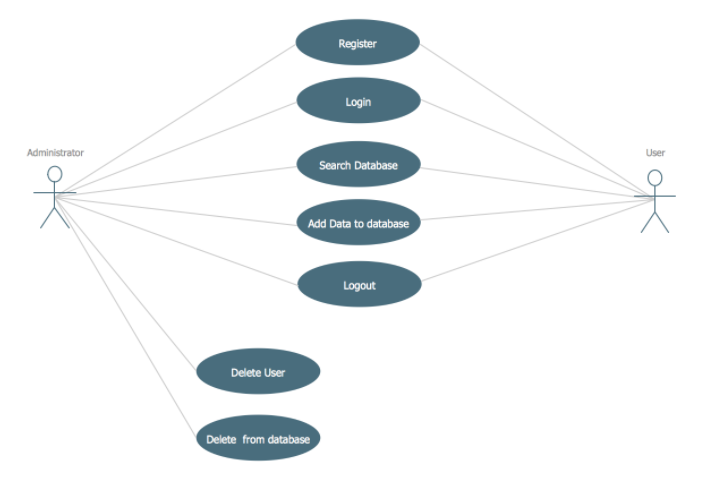
\includegraphics[width=90mm]{system.png}
\caption{Block diagram for the system }
\end{figure}				
		







		

				\subsubsection{User Interfaces}
				
\begin{figure}[!htb]
\minipage{0.32\textwidth}
  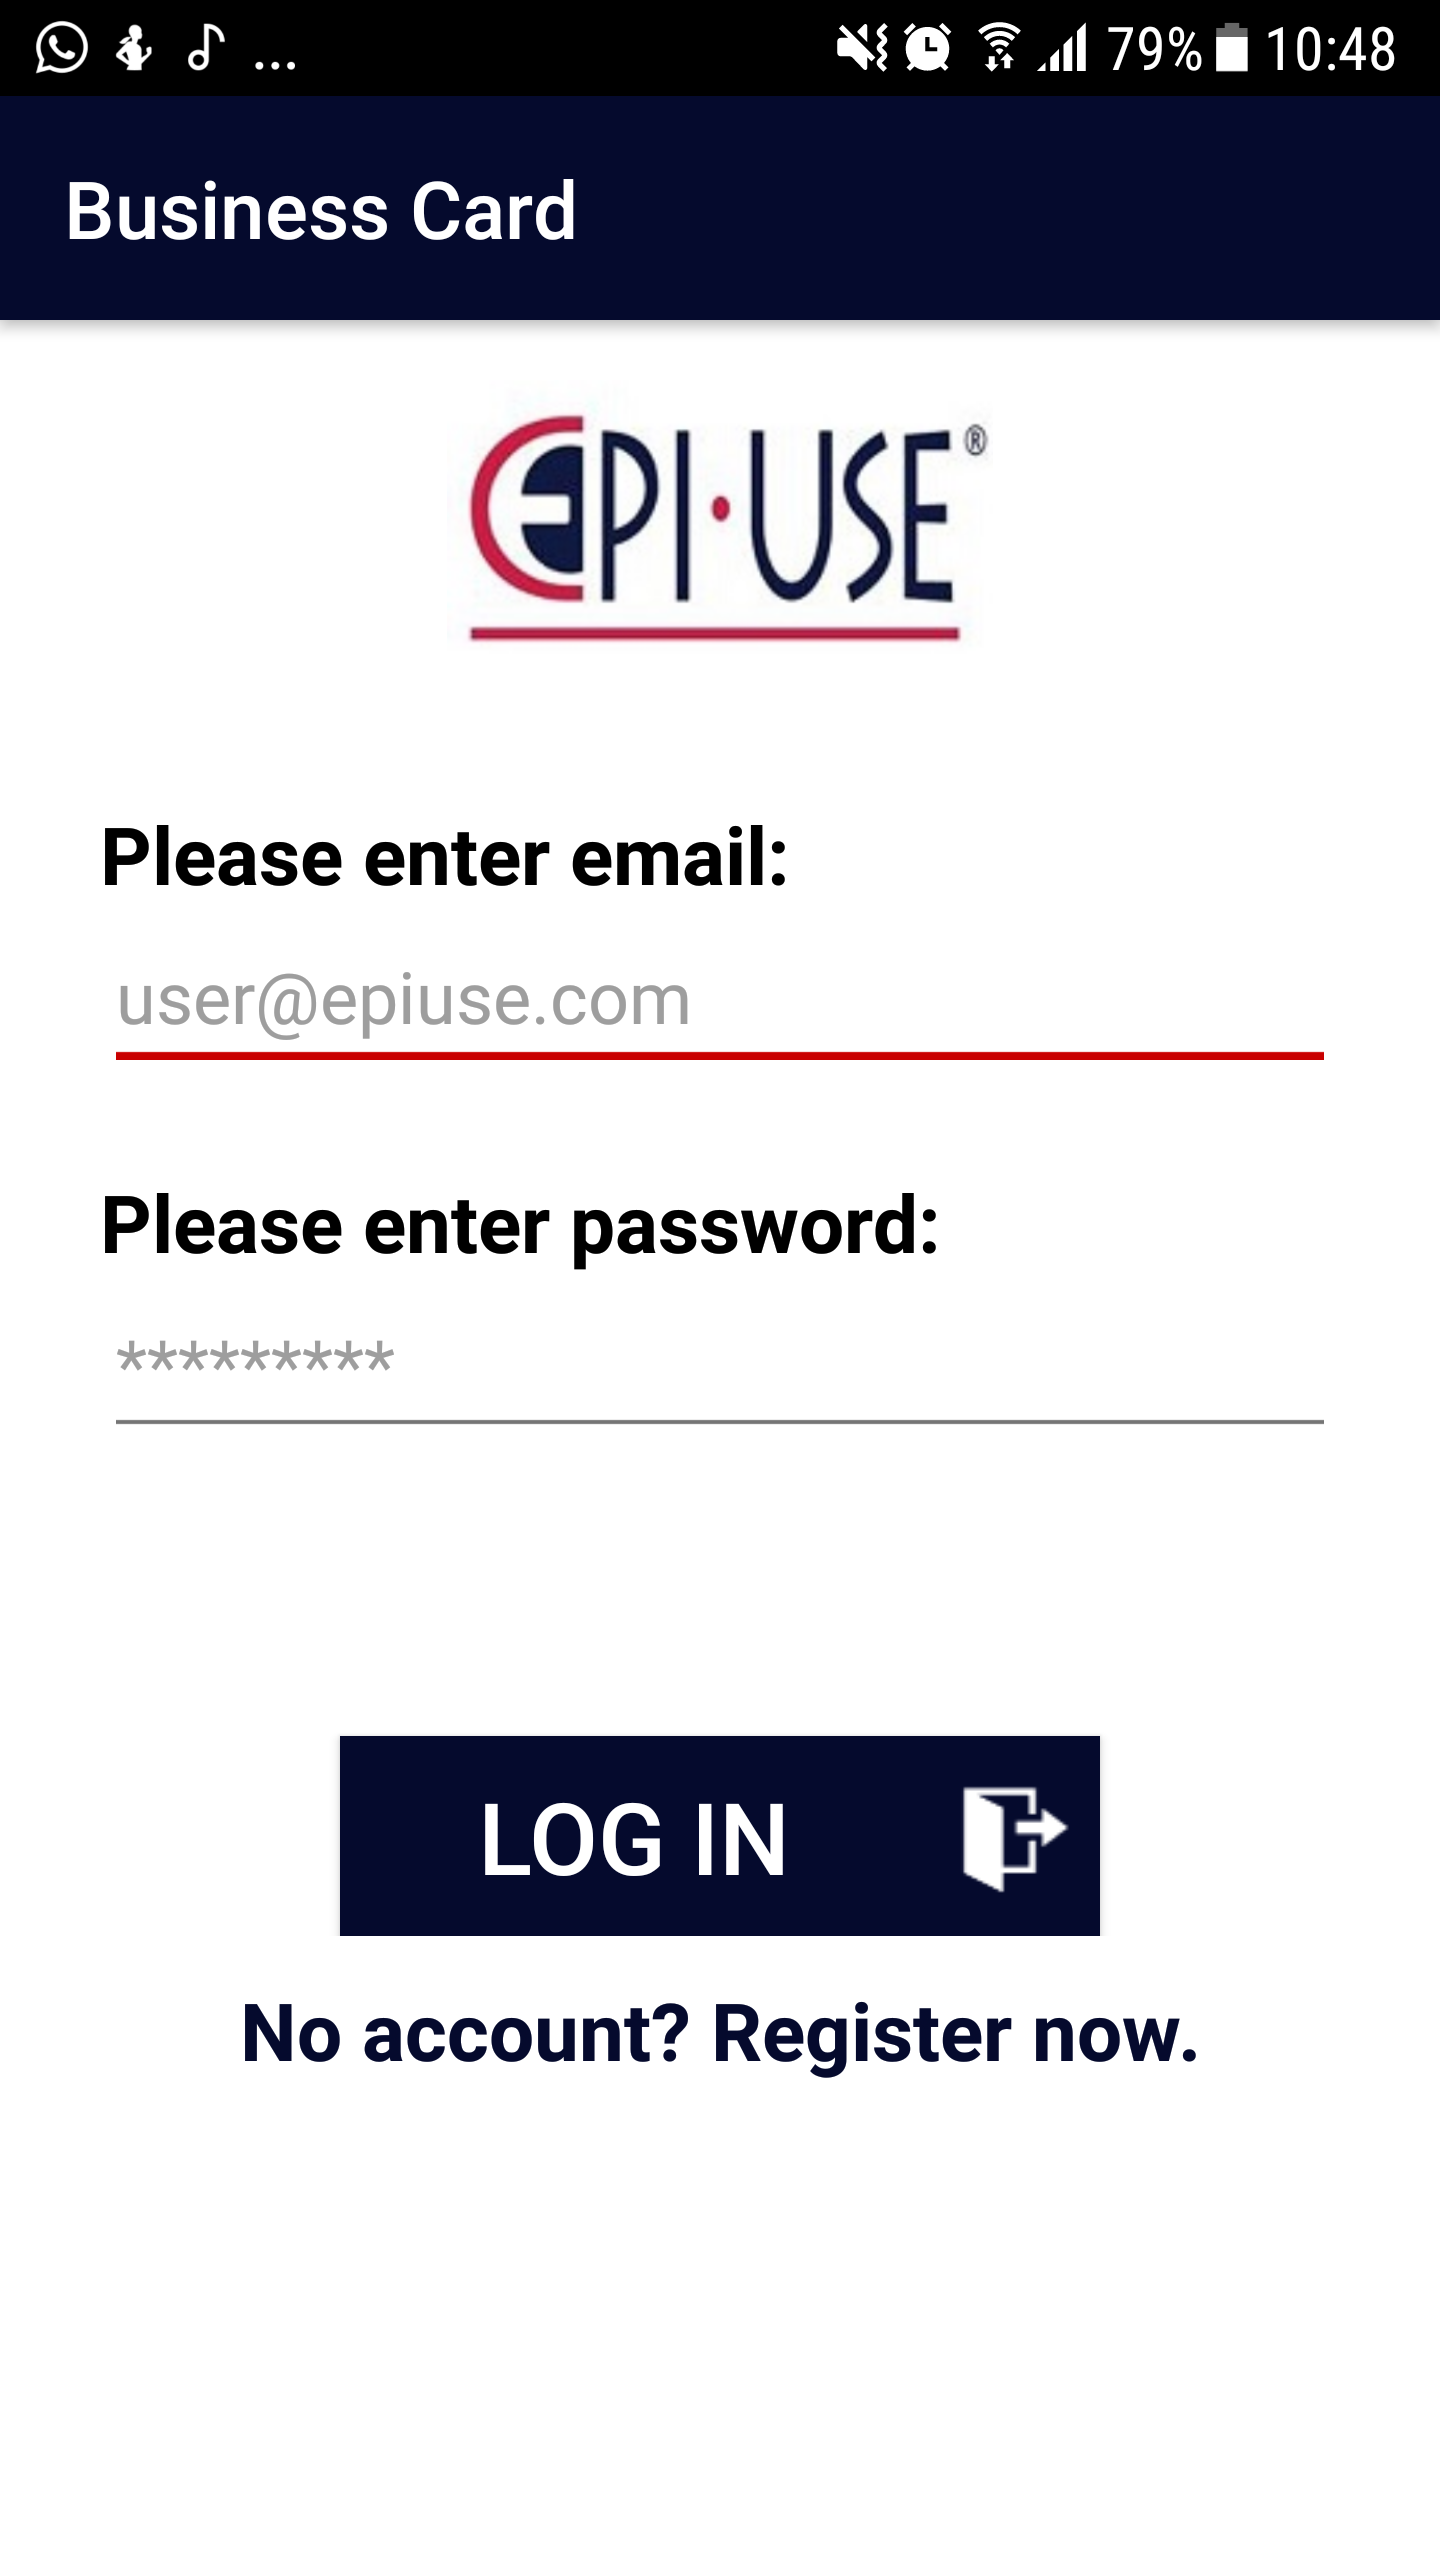
\includegraphics[width=\linewidth]{Login.png}
  \caption{Login}\label{Login}
\endminipage\hfill
\minipage{0.32\textwidth}
  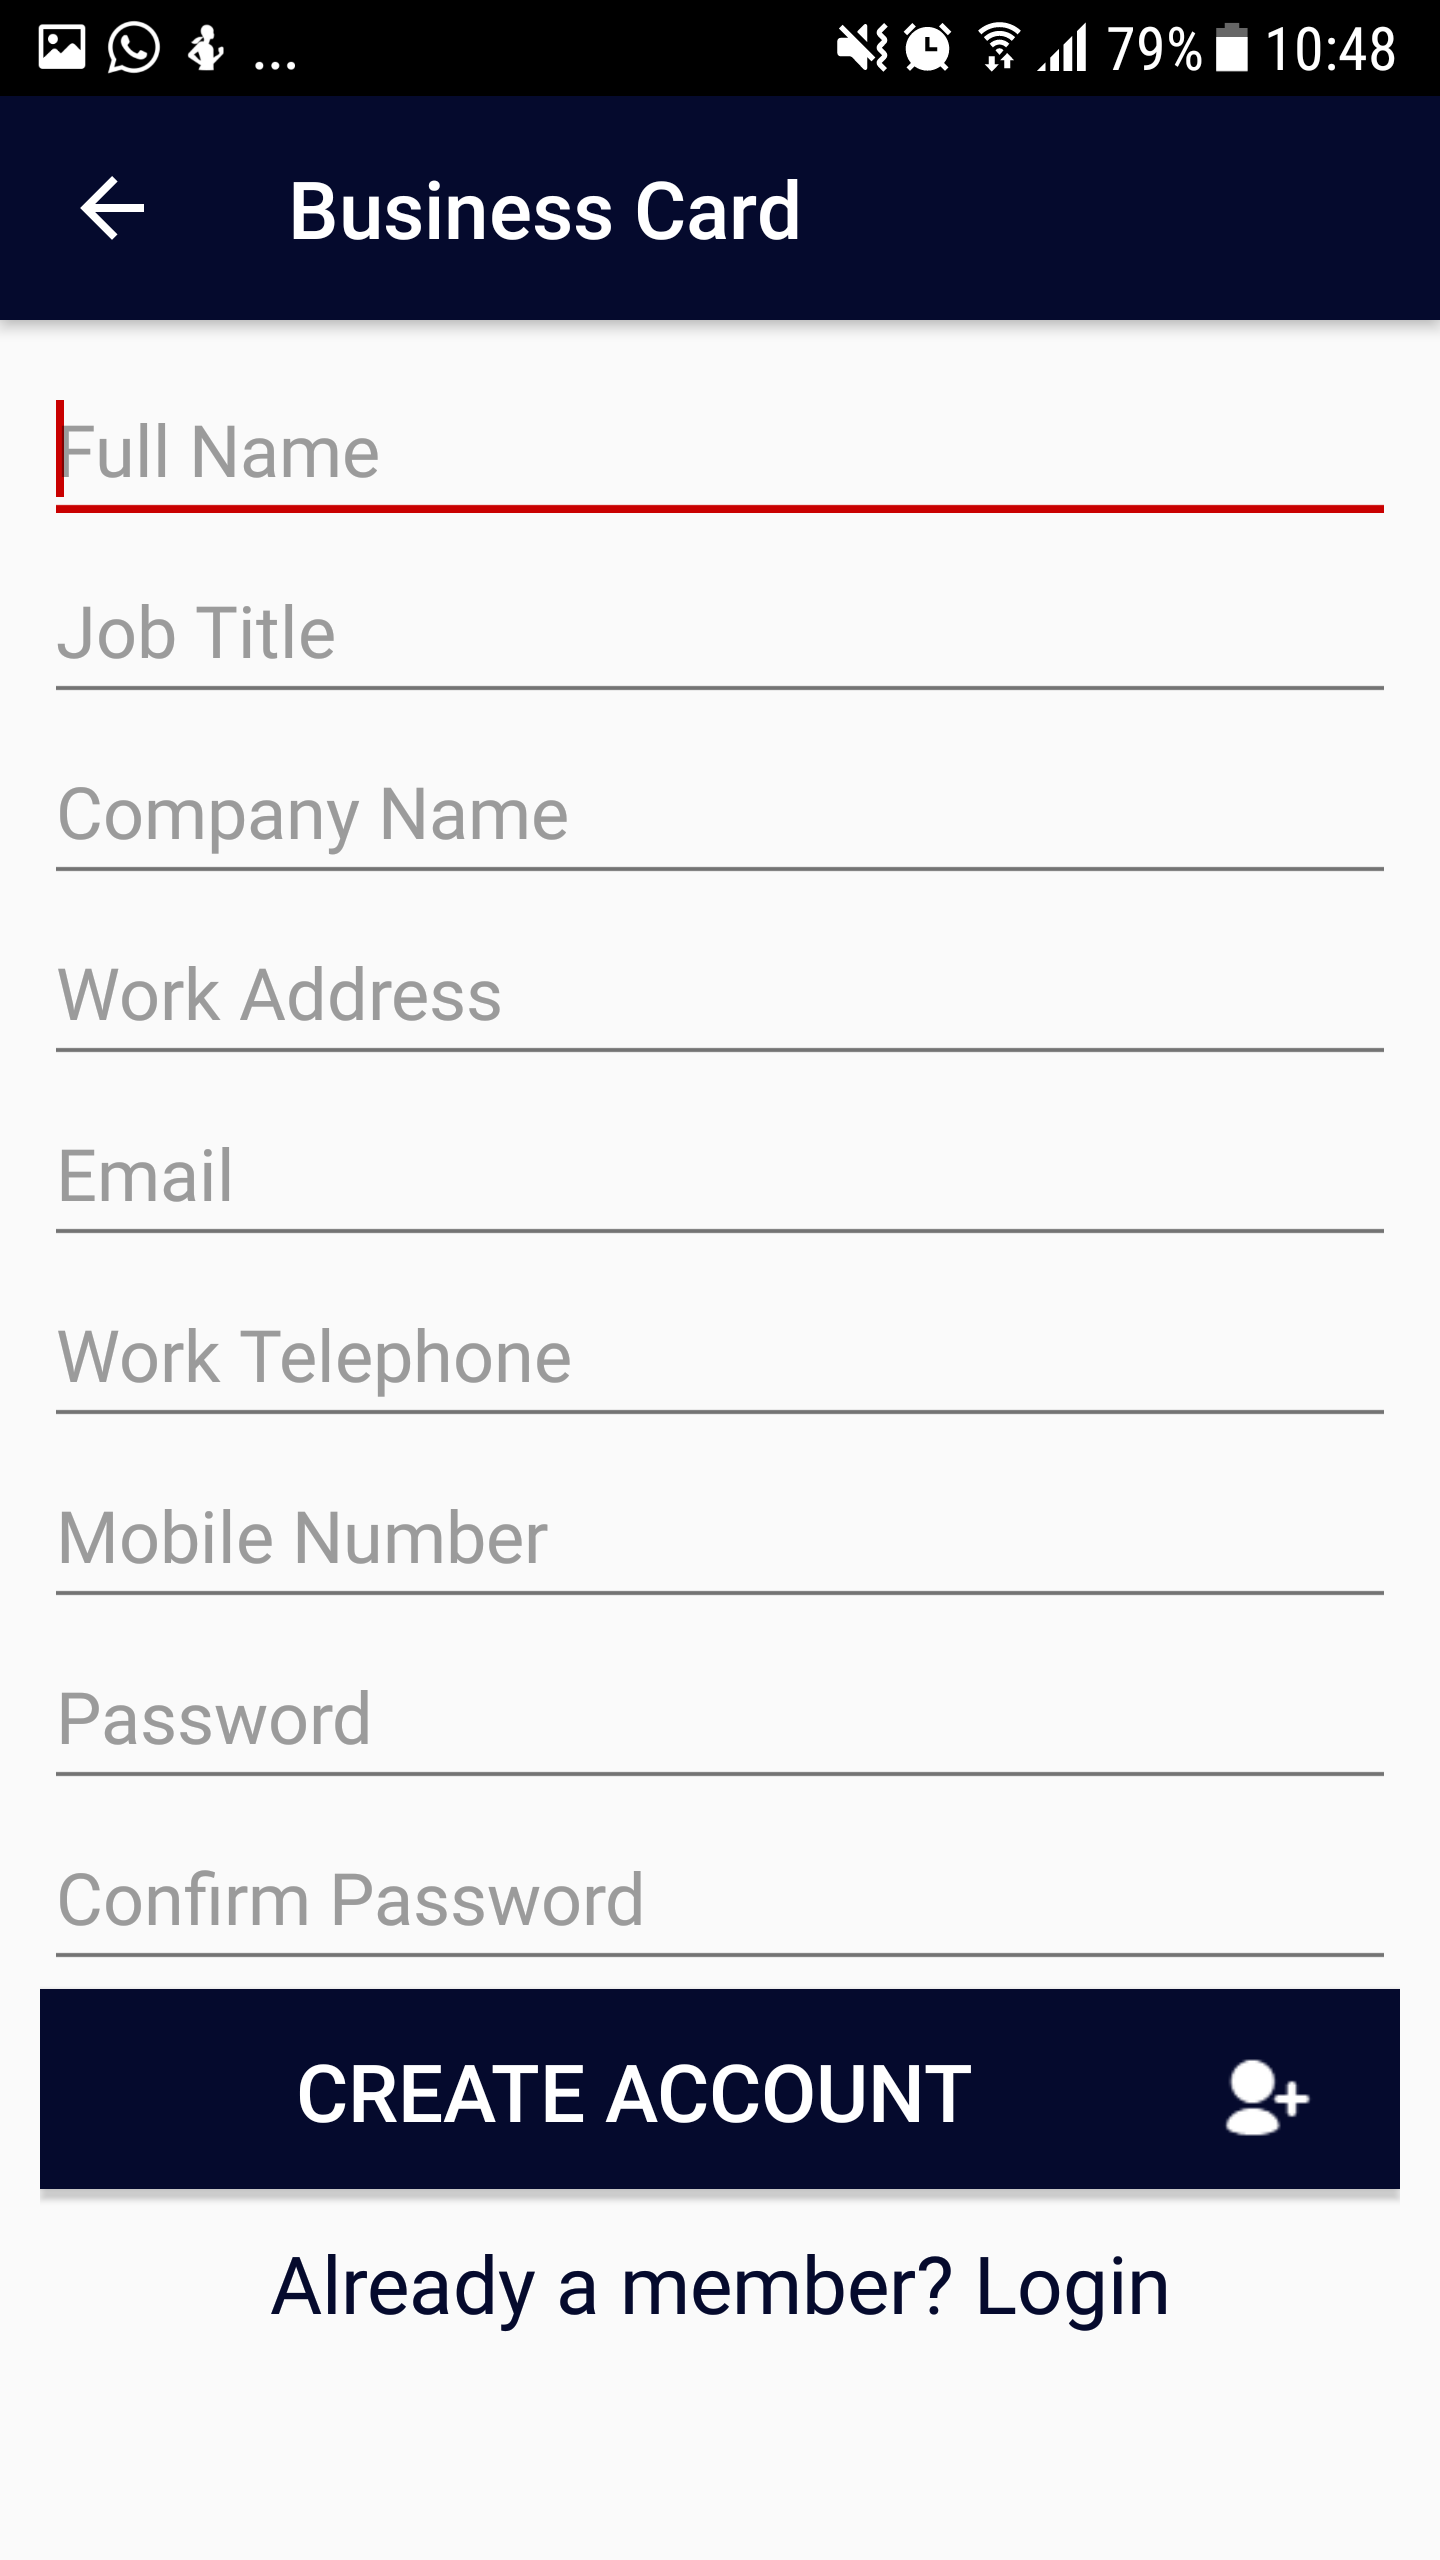
\includegraphics[width=\linewidth]{Register.png}
  \caption{Register}\label{Register}
\endminipage\hfill
\minipage{0.32\textwidth}%
  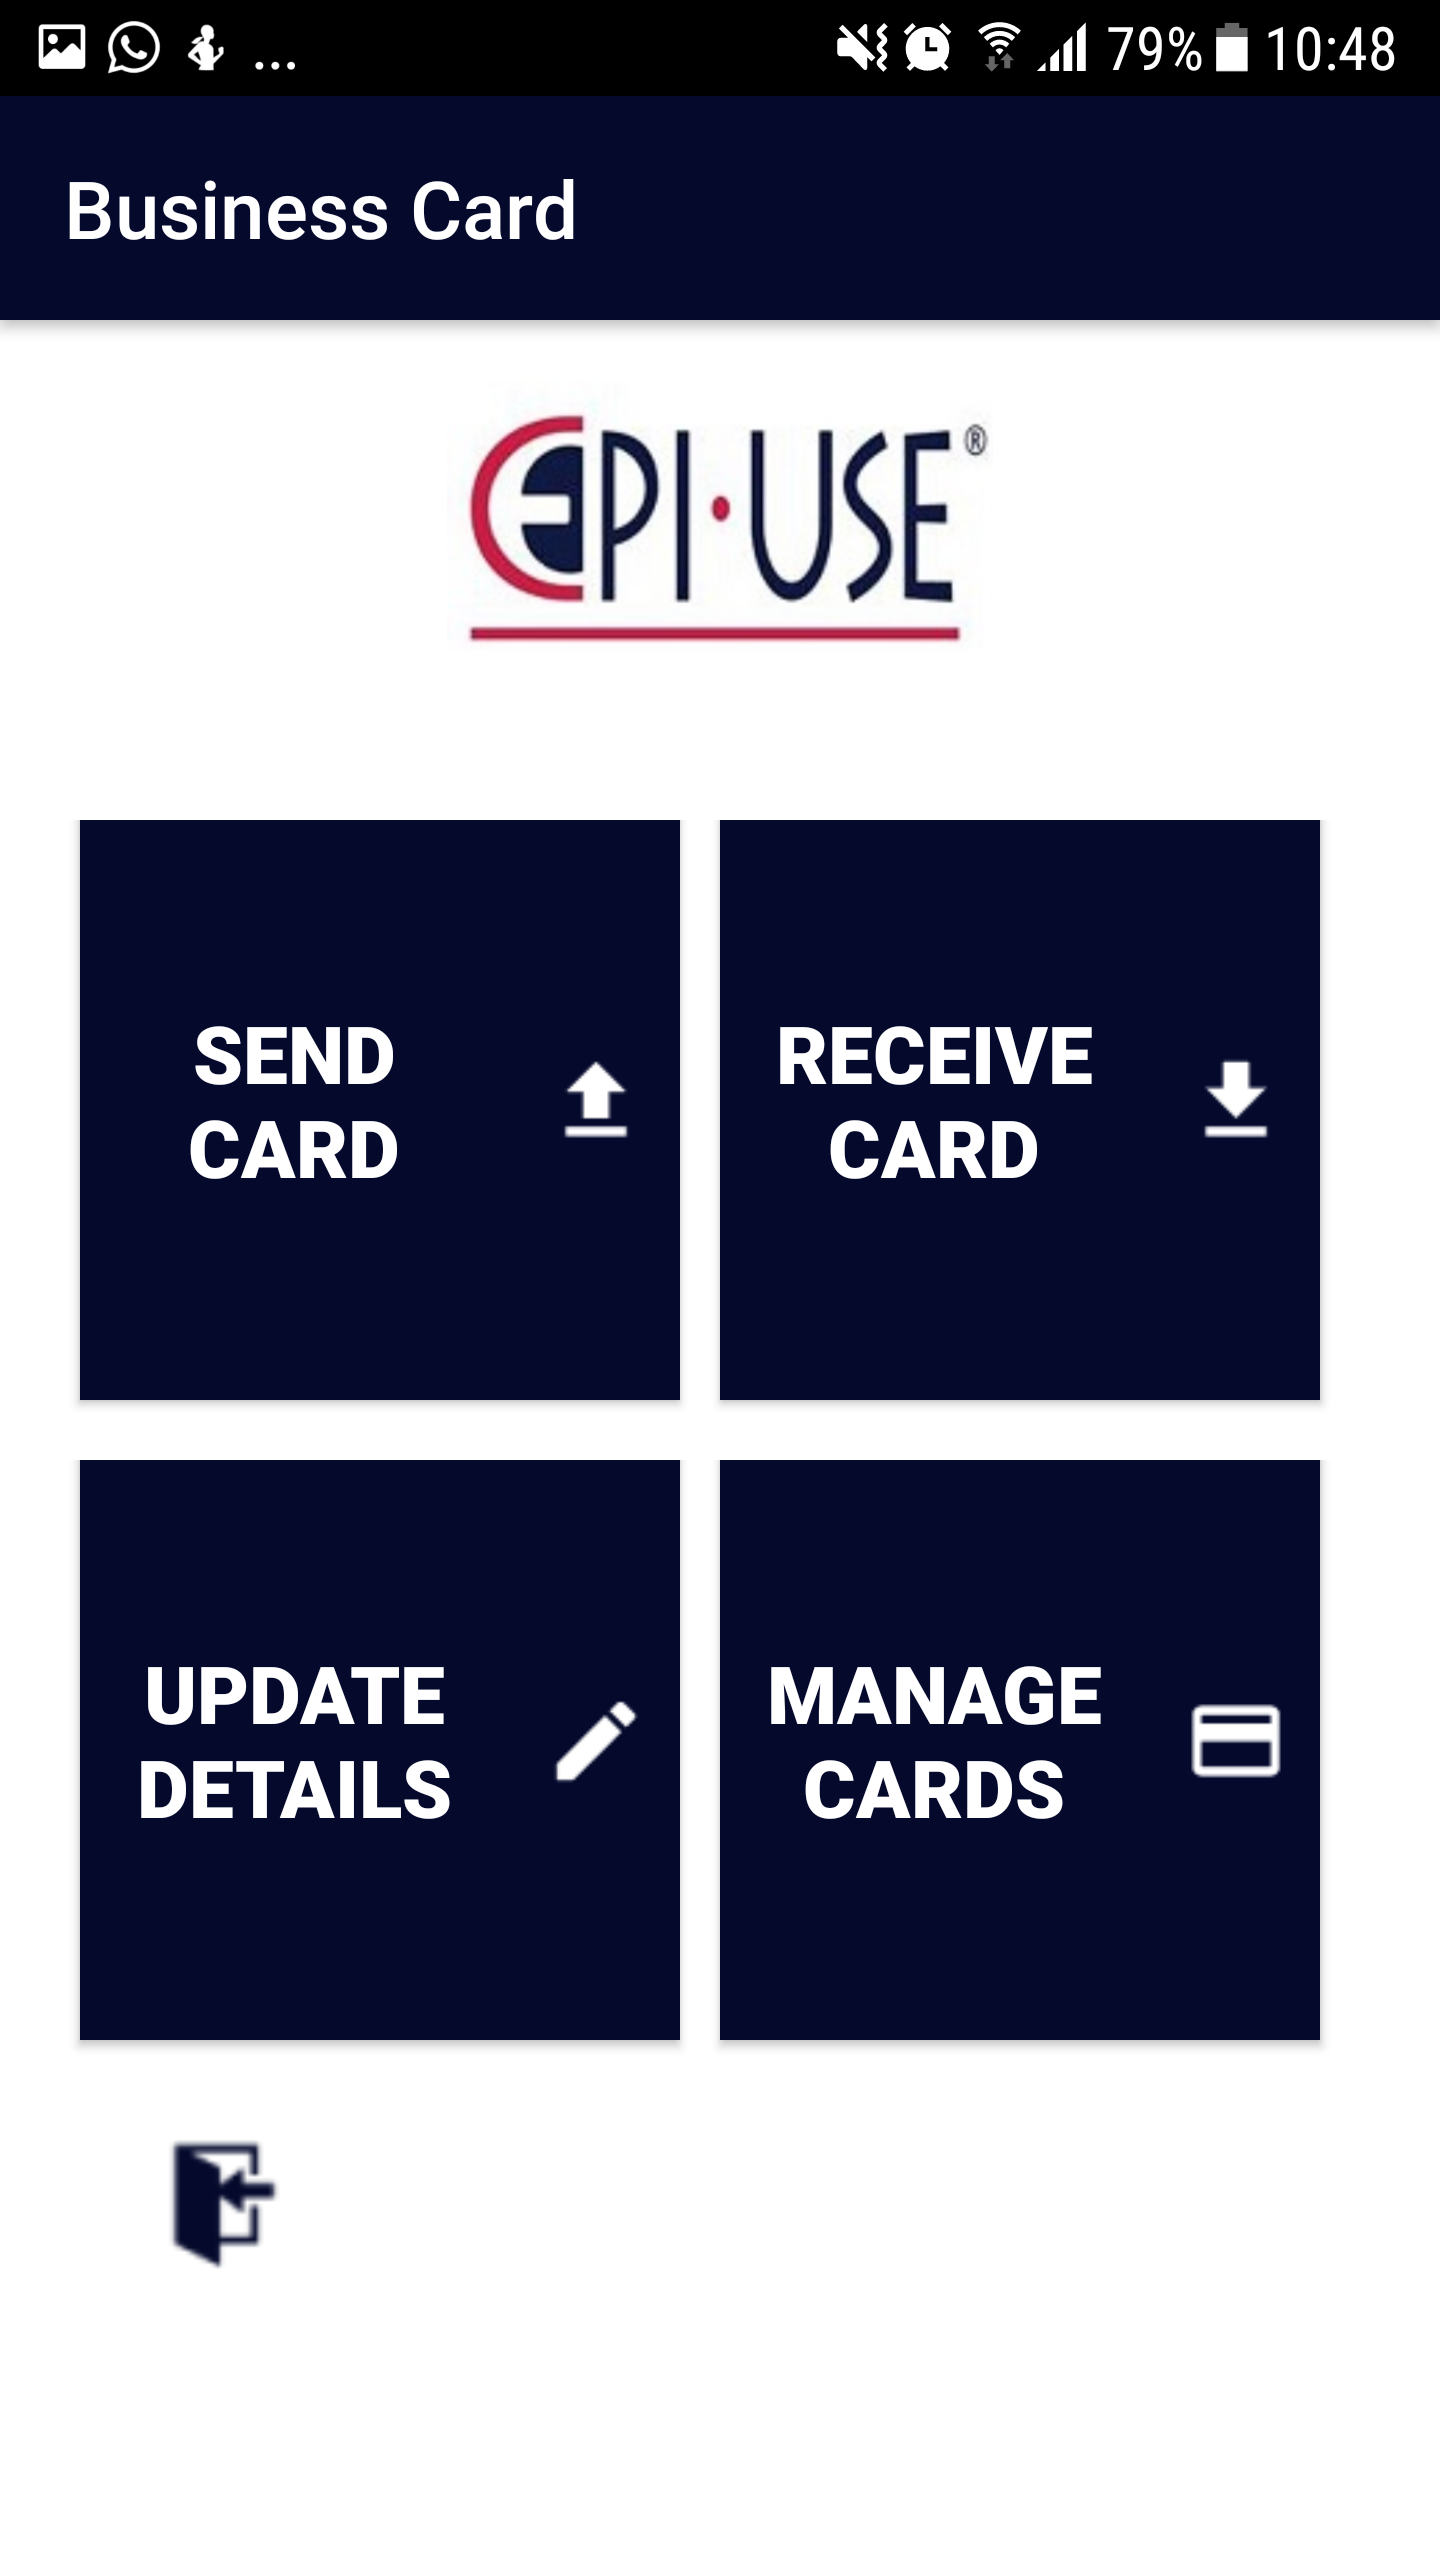
\includegraphics[width=\linewidth]{Main.png}
  \caption{Main}\label{Main}
\endminipage
\end{figure}

								
$\bullet$\ When a user opens the application he/she will see the login page as displayed in figure 1.\\$\bullet$\ If it is a new user then he/she will click on the register link which will then take the user to the register form as shown in figure 2.\\$\bullet$\ After the user successfully registers then the user will be able to see the main page as displayed by figure 3.\\$\bullet$\ The main page shows that the user can be able to send a business card to another user, the user can also receive business cards from other users, the user can update his/her details on the application and also manage the cards which have been received/read from other user.

						

					\subsubsection{Hardware Interfaces}				
$\bullet$\ Devices with NFC will be using the chip on their phones to read from the NFC business card. \\$\bullet$\
The devices which do not have the NFC chip will be using the QR code on the business card to scan the information to the phone.\\$\bullet$\
The web portal will be accessed using a laptop or computer.\\$\bullet$\
The NFC device will be used to read/write to NFC business card.(Check diagram below)\\
\begin{figure}[ht!]
\centering
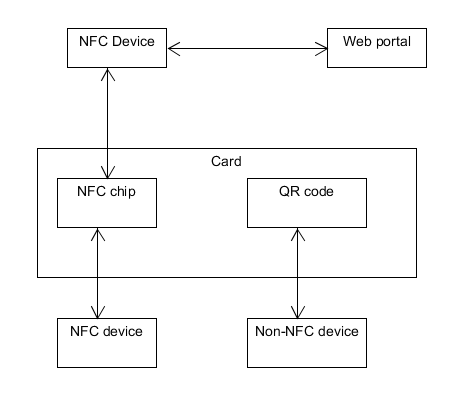
\includegraphics[width=60mm]{Hardware.png}
\caption{Hardware interface block diagram }
\end{figure}

				   
				\subsubsection{Software Interfaces}


\begin{tabular}{ |p{3cm}|p{9cm}|  }
				\hline
				\textbf{} & \textbf{Definition}\\
				\hline
				Cards & Will have both QR and NFC chips embedded on them.\\
				\hline
				Application & Android studios
$\bullet$\ Java
$\bullet$\ Barcode API
$\bullet$\ NFC API
\\
				\hline
				 Web portal & HTML5,CSS,PHP,Javascript\\
				
				\hline
				 Google maps & Google maps API\\
				\hline
				 Database & Firebase database–JSON\\
				\hline
				
				\end{tabular}
\begin{figure}[ht!]
\centering
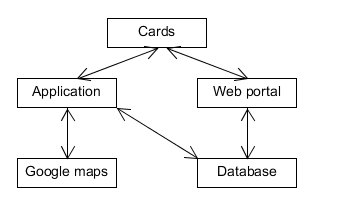
\includegraphics[width=60mm]{Software.png}
\caption{Software interface block diagram}
\end{figure}
			
					
\subsubsection{Communications Interfaces}

\begin{figure}[ht!]
\centering
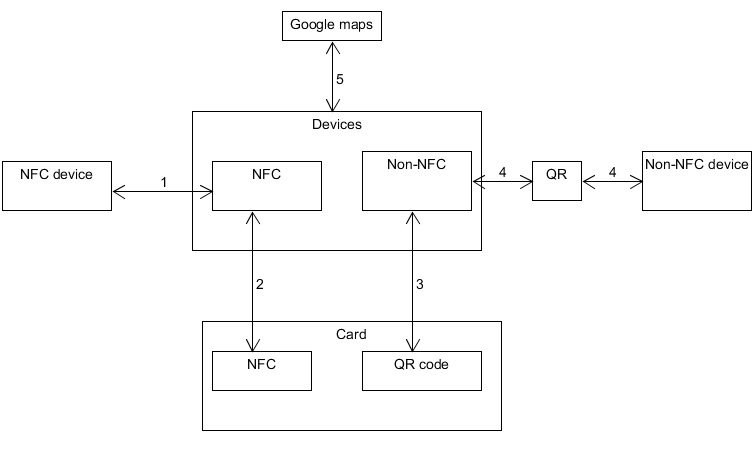
\includegraphics[width=90mm]{communication.png}
\caption{Communication block diagram }
\end{figure}

				1.	NFC Device to NFC device communication\\
$\bullet$\ A phone with an NFC chip exchanging information with another phone having an NFC chip.\\
2.	NFC Device to a NFC business card chip communication\\
$\bullet$\ A phone with NFC chip reading/writing to a NFC business card.\\
3.	Device to QR card communication\\
$\bullet$\ A phone without NFC reading business card which has both NFC chip and QR reader.\\
4.	Device to device communication\\
$\bullet$\ Phone without NFC generating QR code to be read by another phone without NFC.\\
5.	Device connecting to Google maps\\
$\bullet$\ Mobile app communicates with the google maps to get the get the office location of another user.(Check diagram below)


			
				
						\subsubsection{Operations}


\begin{figure}[ht!]
\centering
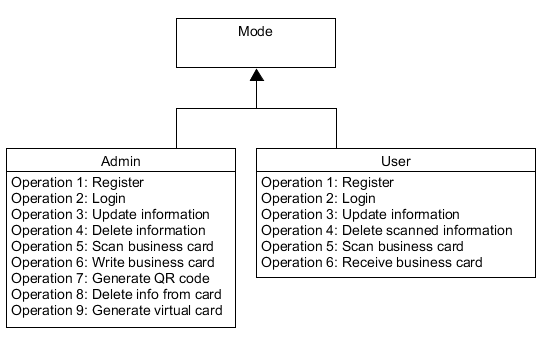
\includegraphics[width=90mm]{operation2.png}
\caption{User mode operations }
\end{figure}				



\begin{figure}[ht!]
\centering
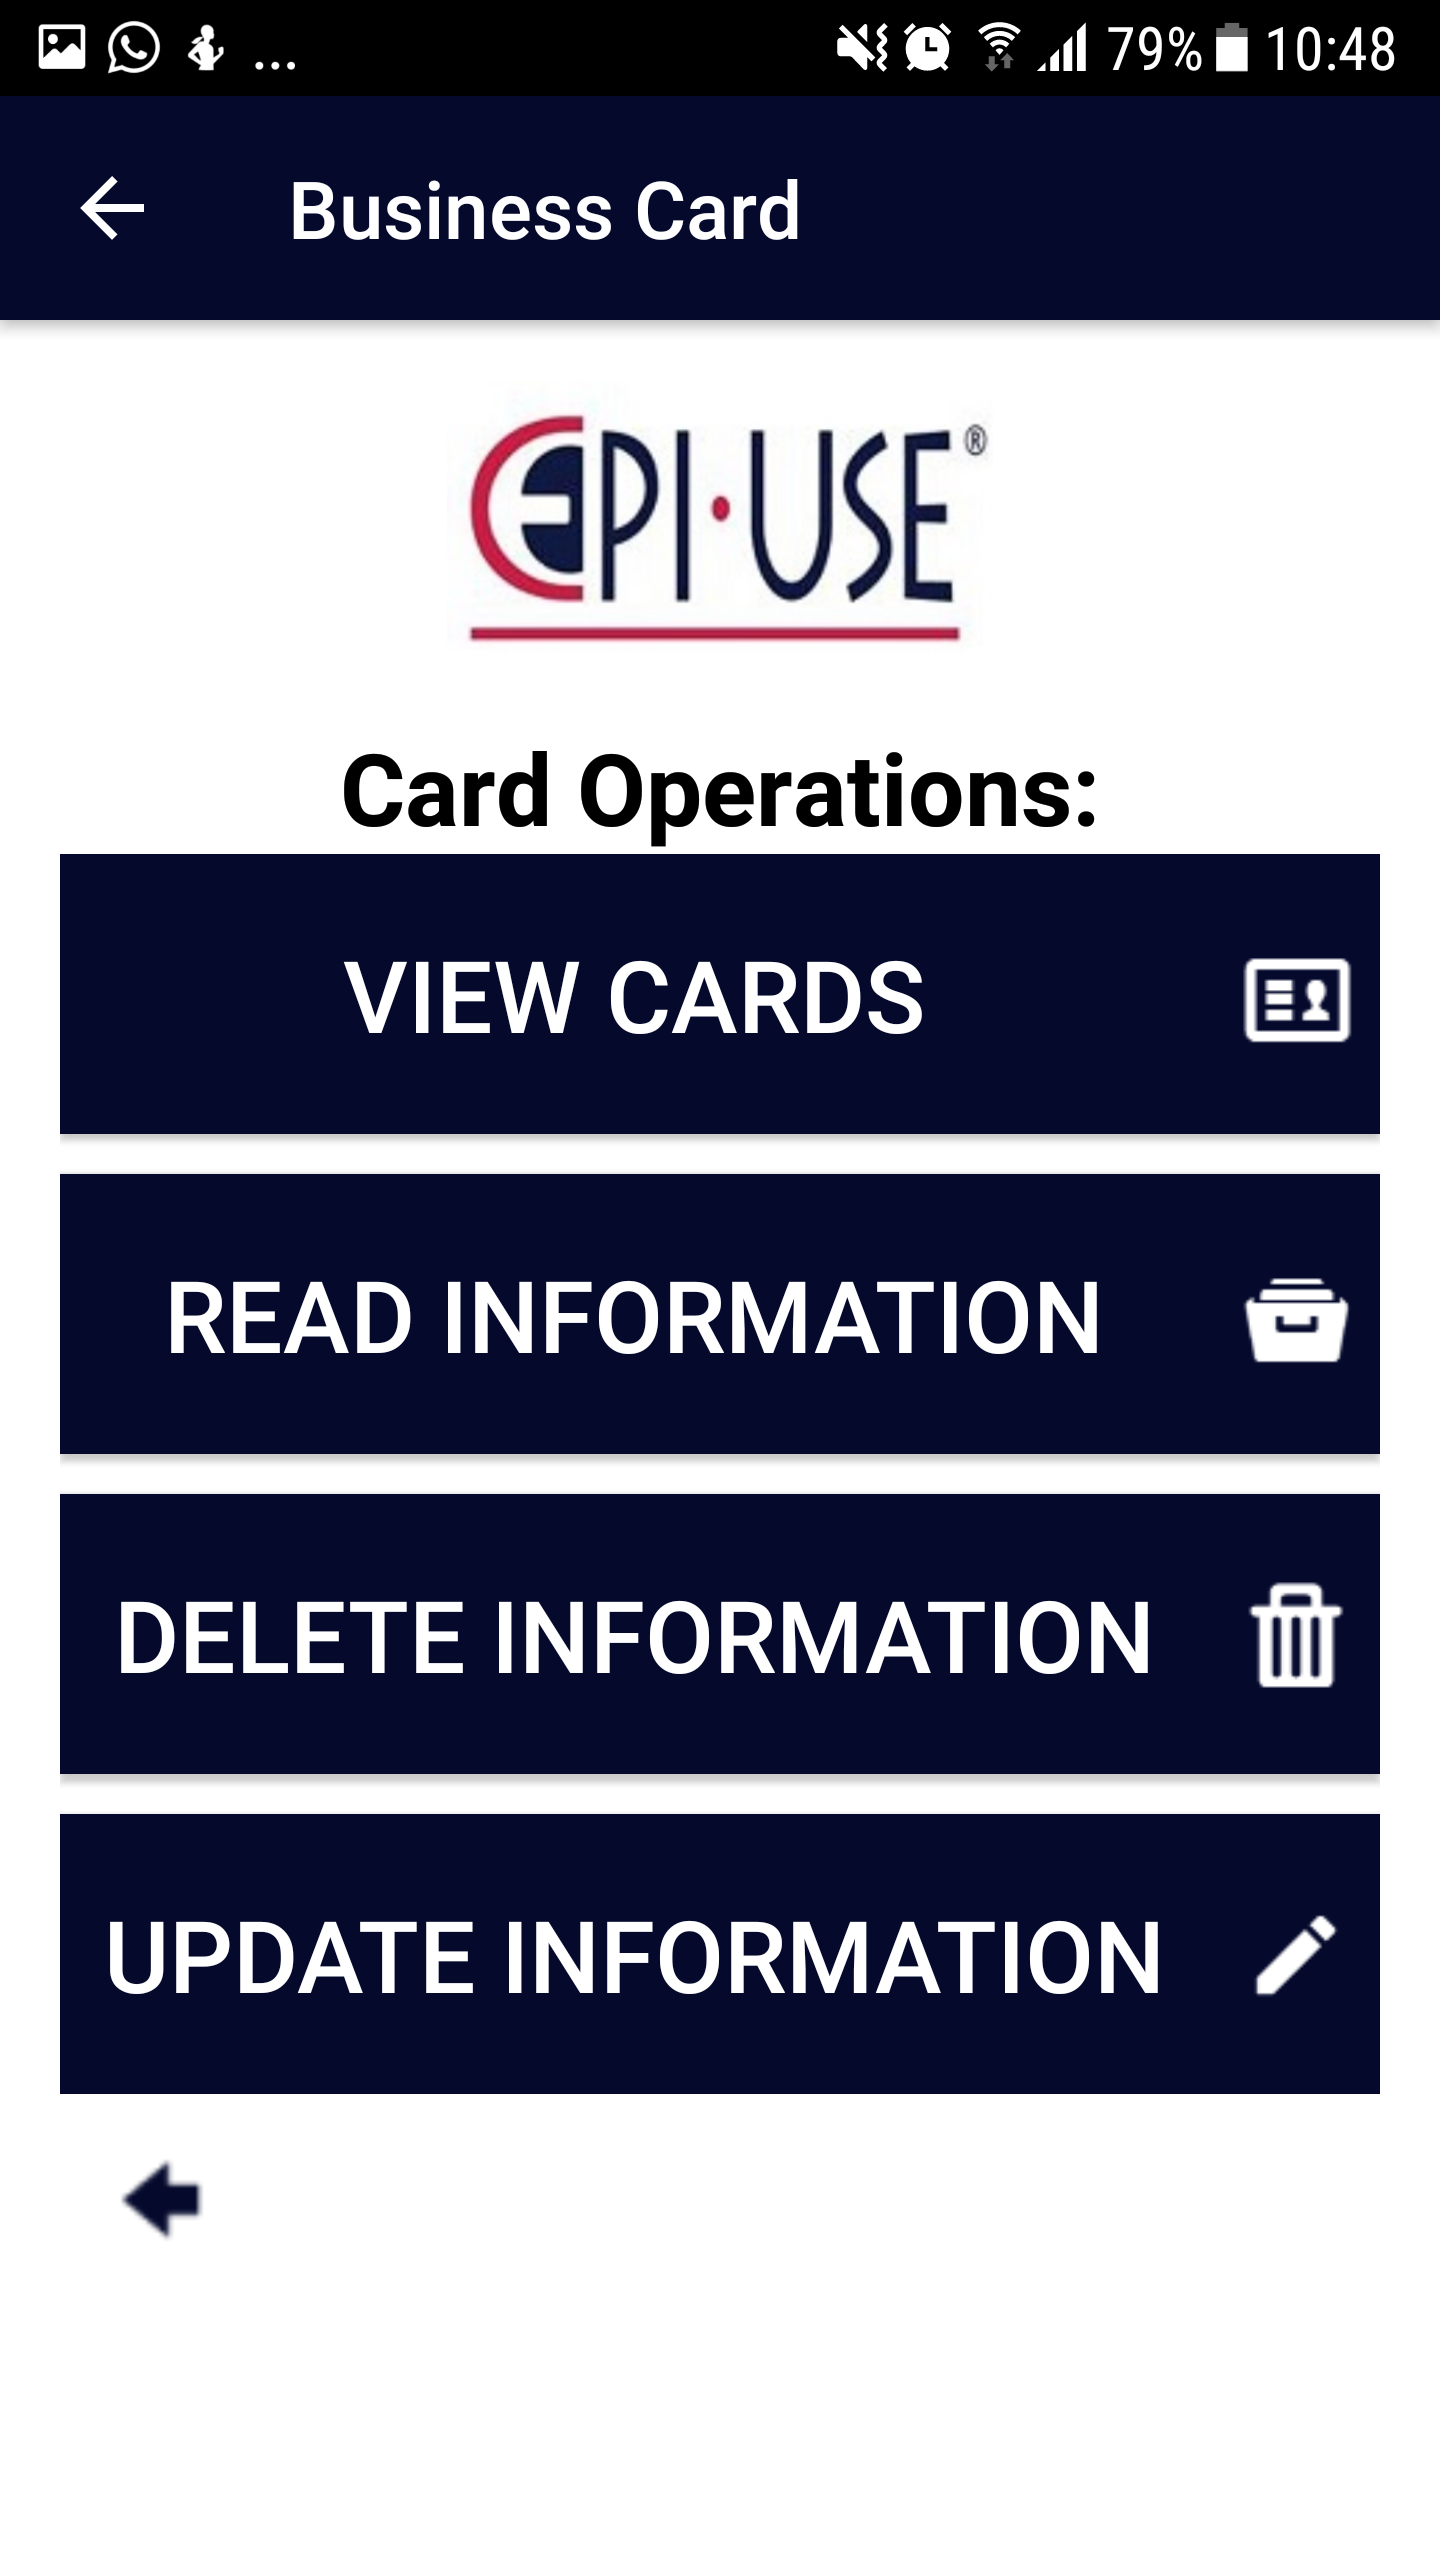
\includegraphics[width=30mm]{operations.png}
\caption{Card Operations }
\end{figure}


$\bullet$\ View cards– User can view the cards which were scanned.
\\$\bullet$\ Delete information- User can decide to delete the details of the cards which were scanned .
\\$\bullet$\ Update information- User can update the information to the card.



				\subsection{Product Functions}

				\subsection{User Characteristics}
				
			
				\subsection{Constraints}
            

				\subsection{Assumptions and Dependencies}
				\subsubsection{Assumptions}


	
				\begin{large}
				\subsubsection{Dependencies}
				\end{large}
		
		\newpage

	\section{Specific Requirements}
				\subsection{External Interface Requirements}
				\subsection{Functional Requirements}
				\subsection{Performance Requirements}
				\subsection{Design Constraints}
				\paragraph\indent
				This application is constrained in two main areas, namely hardware and software. We will look at these two areas separately.
				 \subsubsection{Hardware}
				
				 \subsubsection{Software}
			
				 \subsubsection{Other}
				
					
									\newpage
				\subsection{Software System attributes}
				
				\subsubsection{Reliability}
    			
    				
				\subsubsection{Portability}
 
    				
				\subsubsection{Robustness}
    		
    				
				\subsubsection{Security}
    			
    				
				\subsubsection{Reusability}
	
				    
				\subsubsection{Efficiency}
				  
				\subsubsection{Availability}
				 
	
				\subsubsection{Interoperability}
				

				\subsection{Other Requirements}
				

	
\end{document}
